\let\negmedspace\undefined
\let\negthickspace\undefined
\documentclass[journal]{IEEEtran}
\usepackage[a5paper, margin=10mm, onecolumn]{geometry}
%\usepackage{lmodern} % Ensure lmodern is loaded for pdflatex
\usepackage{tfrupee} % Include tfrupee package

\setlength{\headheight}{1cm} % Set the height of the header box
\setlength{\headsep}{0mm}     % Set the distance between the header box and the top of the text

\usepackage{gvv-book}
\usepackage{gvv}
\usepackage{cite}
\usepackage{amsmath,amssymb,amsfonts,amsthm}
\usepackage{algorithmic}
\usepackage{graphicx}
\usepackage{textcomp}
\usepackage{xcolor}
\usepackage{txfonts}
\usepackage{listings}
\usepackage{enumitem}
\usepackage{mathtools}
\usepackage{gensymb}
\usepackage{comment}
\usepackage[breaklinks=true]{hyperref}
\usepackage{tkz-euclide} 
\usepackage{listings}
\def\inputGnumericTable{}                                 
\usepackage[latin1]{inputenc}                                
\usepackage{color}                                            
\usepackage{array}                                            
\usepackage{longtable}                                       
\usepackage{calc}                                             
\usepackage{multirow}                                         
\usepackage{hhline}                                           
\usepackage{ifthen}                                           
\usepackage{lscape}
\begin{document}

\bibliographystyle{IEEEtran}
\vspace{3cm}

\title{2.2.11}
\author{AI25BTECH11019 - MENAVATH SAI SANJANA}
% \maketitle
% \newpage
% \bigskip
{\let\newpage\relax\maketitle}

\renewcommand{\thefigure}{\theenumi}
\renewcommand{\thetable}{\theenumi}
\setlength{\intextsep}{10pt} % Space between text and floats


\numberwithin{equation}{enumi}
\numberwithin{figure}{enumi}
\renewcommand{\thetable}{\theenumi}

\textbf{Question}:\\
The plane $2x - 3y + 6z - 11 = 0$ makes an angle $\sin^{-1}(\alpha)$ with the x-axis. The value of $\alpha$ is equal to  \\
\\
\bigskip
\textbf{Solution: }

Let the normal vector of the plane be $\overrightarrow{n} = 2\hat{i} - 3\hat{j} + 6\hat{k}$.

The x-axis has direction vector $\overrightarrow{a} = \hat{i}$.

The cosine of the angle $\theta$ between the normal and x-axis:
$
\cos\theta = \frac{\overrightarrow{n} \cdot \overrightarrow{a}}{|\vec{n}| \cdot |\vec{a}|}
\\ = \frac{2}{\sqrt{2^2 + (-3)^2 + 6^2}} = \frac{2}{7}
$
\bigskip
Angle between plane and x-axis $= 90^\circ - \theta$.

Thus,
$
\alpha = \sin(90^\circ - \theta) = \cos\theta = \frac{2}{7}
$
So, the value of $\alpha$ is $2/7$.


\begin{figure}[ht!]
    \centering
    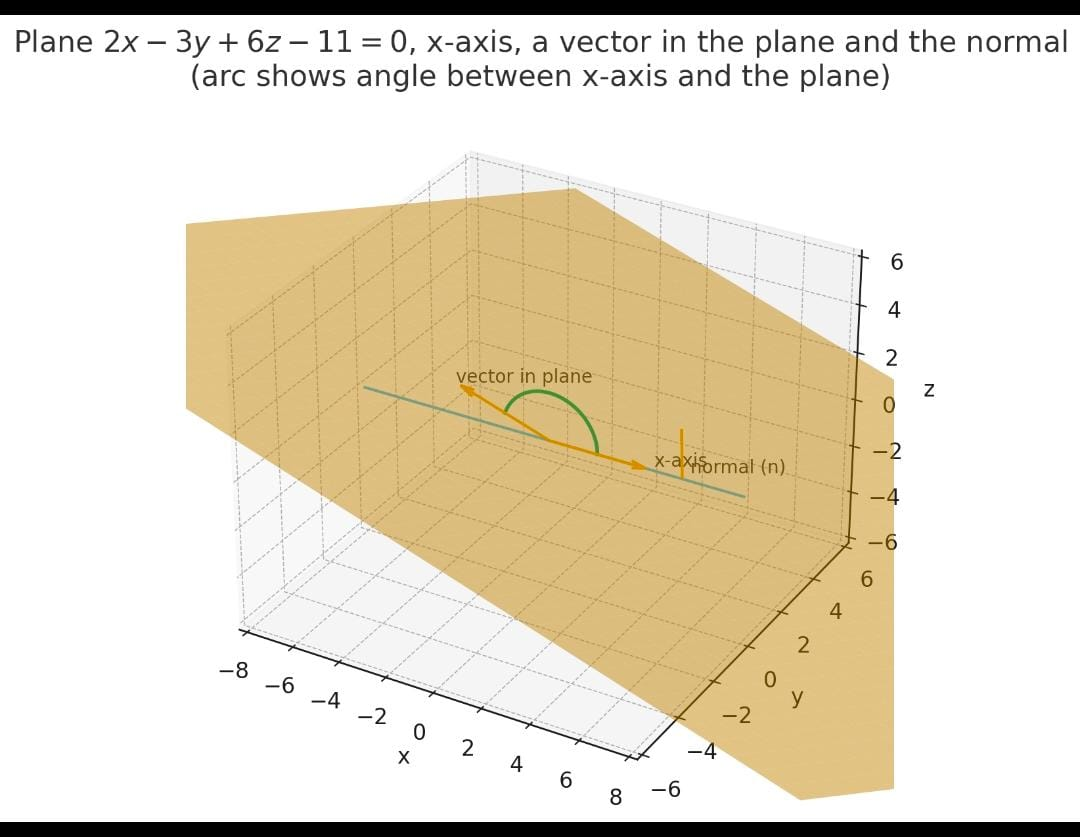
\includegraphics[width=0.8\textwidth]{figs/matgeo-2.2.11.jpeg}
    \caption{}
    \label{fig:1.2.27.jpg}
\end{figure}

\end{document}
